
Muchos sitios web intentan comparar las preferencias de dos usuarios para realizar sugerencias a partir de las preferencias de usuarios con gustos similares a los nuestros. Dado un ranking de $n$ productos (p.ej. pel\'iculas) mediante el cual los usuarios indicamos nuestras preferencias, un algoritmo puede medir la similitud de nuestras preferencias contando el n\'umero de inversiones: dos productos $i$ y $j$ est\'an \"invertidos\" en las preferencias de $A$ y $B$ si el usuario $A$ prefiere el producto $i$ antes que el $j$, mientras que el usuario $B$ prefiere el producto $j$ antes que el $i$. Esto es, cuantas menos inversiones existan entre dos rankings, m\'as similares ser\'an las
preferencias de los usuarios representados por esos rankings.

Por simplicidad podemos suponer que los productos se pueden identificar mediante enteros
$1, \cdots, n$, y que uno de los rankings siempre es $1,\cdots, n$ (si no fuese as\'i bastar\'ia reenumerarlos) y el otro es $a_1, a_2, \cdots, a_n$, de forma que dos productos $i$ y $j$ est\'an invertidos si $i < j$ pero $a_i > a_j$.
De esta forma nuestra representaci\'on del problema ser\'a un vector de enteros $v$ de tamaño $n$, de forma que $v[i] = a_i\ / \ i = 1, \cdots, n$.

El objetivo es diseñar, analizar la eficiencia e implementar un algoritmo \"divide y vencer\'as\" para medir la similitud entre dos rankings. Compararlo con el algoritmo de \"fuerza bruta\" obvio. Realizar tambi\'en un estudio emp\'irico e h\'ibrido de la eficiencia de ambos algoritmos.

\subsection{Fuerza bruta}
La aproximación mas natural al problema sería comparar cada elemento del vector con todos los demás, aunque realmente solo es necesario hacer la comparación con los elementos que están por delante (tienen mayor índice) en el vector.\\

\textbf{Ejemplo:}

\begin{center}
\fcolorbox{gray75}{gray97}{
\begin{tabular}{|c|c|c|c|}
\hline
3 & 4 & 2 & 1\\
\hline
\end{tabular}
}
\end{center}

\begin{itemize}
\item 3 no está invertido con 4
\item 3 está invertido con 2
\item 3 está invertido con 1
\item 4 está invertido con 2
\item 4 está invertido con 1
\item 2 está invertido con 1
\end{itemize}

\subsubsection{Eficiencia teórica}
La eficiencia del algoritmo viene dada por el número de comparaciones que realiza en relación al tamaño del vector.\\

Tomando $n \equiv Tamaño\ del\ vector$ tenemos que:\\

$$Num\ de\ comparaciones = \sum_{i=1}^{n-1}n-i = n(n-1) - \sum_{i=1}^{n-1}i = n(n-1) - \frac{n^2 - n}{2} = \frac{n^2 - n}{2} \longrightarrow O(n^2)$$

Deducimos así que nuestro algoritmo es de orden cuadrático.\\

\subsubsection{Eficiencia empírica}
Para medir la eficiencia empírica hemos implementado el algoritmo en \textit{fuerza\_bruta.cpp}\\

Al utilizar el algoritmo con vectores de distintos tamaños hemos obtenido \hyperref[tabla_comp]{{\color{blue} los siguientes tiempos}}\\

Visto en forma de gráfica se puede apreciar la relación cuadrática que habíamos deducido en el apartado anterior.\\

La función utilizada en el ajuste es $f(n) = an^2 + bn + c$

Los resultados del ajuste son:\\

\begin{center}
\fcolorbox{gray75}{gray97}{
	$a = 4.62037 \cdot 10^{-9}$ , $b = 7.56764 \cdot 10^{-9}$ , $c = -3.85366 \cdot 10^{-5}$
}
\end{center}


\begin{figure}[h]
\centering
	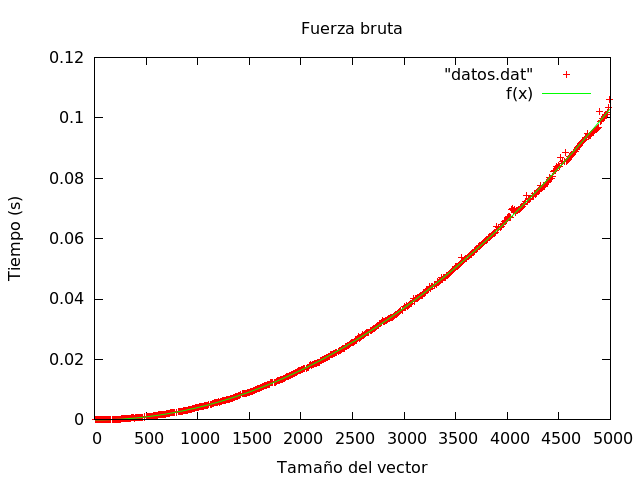
\includegraphics[width=0.6\textwidth]{../Opcional/Graficas/fuerza_bruta_bruno.png}
	\caption{Gráfica fuerza bruta} 
	\label{fig:perros} 
\end{figure}

\newpage

\subsection{Divide y vencerás}
Para realizar la versión divide y vencerás del algoritmo hemos utilizado el método de mezcla.\\

Primero dividimos el vector en trozos, los cuales comparamos unos con otros (de la misma forma que en el algoritmo anterior) al mezclarlos.\\


\begin{figure}[h] 
\centering
	\fcolorbox{gray75}{gray97}{
	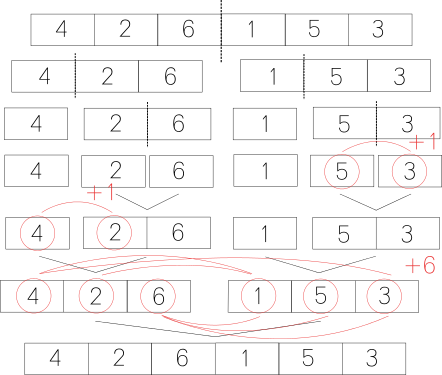
\includegraphics[width=0.5\textwidth]{Imagenes/esquema.png}
	}
	\caption{Ejemplo} 
\end{figure}


\subsubsection{Eficiencia teórica}
La forma natural de plantear la eficiencia teórica es como una ecuación en recurrencia:\\

$$\left\lbrace
	\begin{array}{l}
	T(n) = \frac{n^2 - n}{2}\  si\ n \leq 2\\
	T(n) = 2T(\frac{n}{2}) + 2n\  si\ n > 2 \\
	\end{array}
	\right.$$\\
	
Donde el $2n$ de la segunda ecuación representa el cose de unir las dos partes del vector.\\

Desarrollando la recurrencia mediante cambio de variable tenemos que:\\

$$n=2^k \Rightarrow k = \log_2n$$
$$T(2^k) = 2T(2^{k-1}) + 2^{k+1}$$\\

Cuyo polinomio característico es $p(\lambda) = (\lambda - 2)^2$\\
La solución de la ecuación es:\\
$$T(k)=c_12^k+c_2k2^k \Rightarrow T(n) = n^2(c_1+c_2\log_2n)$$

Para obtener $c_1$ y $c_2$ utilizamos que:

$$\left\lbrace
	\begin{array}{l}
	T(1) = c_1 = 0\\
	T(2) = 4(c_1 + c_2) = 1\\
	\end{array}
	\right. \Rightarrow c_1 = 0, c_2 = \frac{1}{4}$$\\
	
Por tanto $T(n) = \frac{1}{4}n^2\log_2n \longrightarrow O(n^2\log_2n)$
	

\subsubsection{Eficiencia empírica}
Para medir la eficiencia empírica hemos implementado el algoritmo en \textit{dyv.cpp}\\

Al utilizar el algoritmo con vectores de distintos tamaños hemos obtenido \hyperref[tabla_comp]{{\color{blue} los siguientes tiempos}}\\

Visto en forma de gráfica se puede apreciar la relación cuadrática que habíamos deducido en el apartado anterior.\\

La función utilizada en el ajuste es $f(n) = an^2 \cdot \log_2n)$

Los resultados del ajuste son:\\

\begin{center}
\fcolorbox{gray75}{gray97}{
	$a = 2.6999 \cdot 10^{-9}$
}
\end{center}

Como se puede ver mejoramos el tiempo respecto a la fuerza bruta.

\begin{figure}[h] 
\centering
	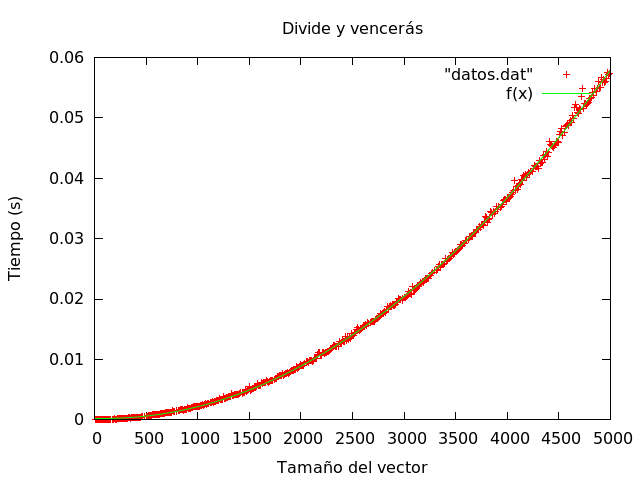
\includegraphics[width=0.6\textwidth]{../Opcional/Graficas/dyv_bruno.png}
	\caption{Gráfica DyV} 
	\label{fig:perros} 
\end{figure}


\subsection{Divide y vencerás con mergesort}
Una mejor forma de implementar divide y vencerás es utilizar el algoritmo de ordenación mergesort. La ventaja respecto al anterior es que, estando el vector ordenado, sabemos que si un elemento esta invertido con otro de la sección izquierda del vector, también lo estarán todos los que le siguen (al ser mayores).

\begin{figure}[h] 
\centering
	\fcolorbox{gray75}{gray97}{
	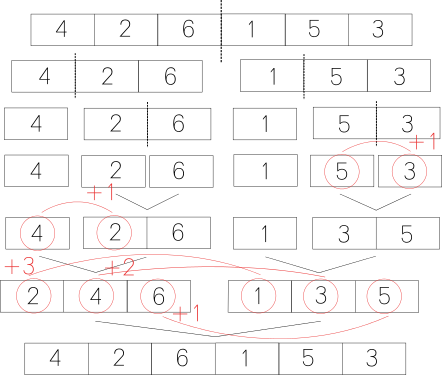
\includegraphics[width=0.5\textwidth]{Imagenes/esquema_merge.png}
	}
	\caption{Ejemplo} 
\end{figure}

\subsubsection{Eficiencia teórica}
Al utilizar mergesort la eficiencia es $nlog(n)$

\subsubsection{Eficiencia empírica}
Para medir la eficiencia empírica hemos implementado el algoritmo en \textit{dyv\_mergesort.cpp}\\

Al utilizar el algoritmo con vectores de distintos tamaños hemos obtenido \hyperref[tabla_comp]{{\color{blue} los siguientes tiempos}}\\

Visto en forma de gráfica se puede apreciar el orden n-logarítmico que habíamos deducido en el apartado anterior.\\

La función utilizada en el ajuste es $f(n) = a \cdot n \cdot log_2(n)$

Los resultados del ajuste son:\\

\begin{center}
\fcolorbox{gray75}{gray97}{
	$a = 1.99872 \cdot 10^{-8}$
}
\end{center}

De esta forma conseguimos reducir el orden del algoritmo con la aproximación divide y vencerás.

\begin{figure}[h] 
\centering
	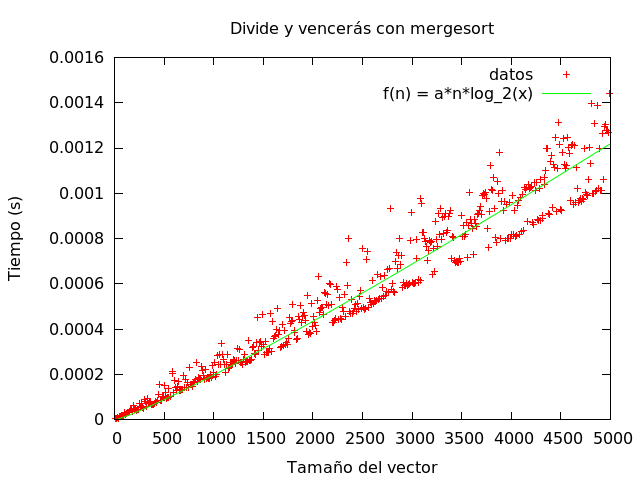
\includegraphics[width=0.6\textwidth]{../Opcional/Graficas/dyv_mergesort_bruno.png}
	\caption{Gráfica DyV mergesort} 
	\label{fig:perros} 
\end{figure}
\newpage

\subsection{Comparación}
Al comparar los datos se puede ver la diferencia de velocidad entre los algoritmos\\

\label{tabla_comp}
\begin{center}
\begin{longtable}{l|l|l|l}
\multicolumn{1}{c}{\textbf{N}} & \multicolumn{1}{c}{\textbf{FUERZA BRUTA}} & \multicolumn{1}{c}{\textbf{DyV}} & \multicolumn{1}{c}{\textbf{DyV MERGESORT}} \\
\hline
10                                                     & 5.372e-06                                                         & 5.01e-06                                                 & 4.475e-06                                                          \\
20                                                     & 8.789e-06                                                         & 1.7346e-05                                               & 4.593e-06                                                          \\
30                                                     & 7.569e-06                                                         & 8.699e-06                                                & 6.213e-06                                                          \\
40                                                     & 1.0783e-05                                                        & 1.6202e-05                                               & 1.2129e-05                                                         \\
50                                                     & 1.7045e-05                                                        & 1.9298e-05                                               & 1.3067e-05                                                         \\
60                                                     & 2.1477e-05                                                        & 1.8845e-05                                               & 1.1179e-05                                                         \\
70                                                     & 2.6556e-05                                                        & 2.3171e-05                                               & 1.2893e-05                                                         \\
80                                                     & 3.3474e-05                                                        & 2.9005e-05                                               & 1.43e-05                                                           \\
90                                                     & 3.8403e-05                                                        & 3.9902e-05                                               & 2.0181e-05                                                         \\
100                                                    & 4.3868e-05                                                        & 4.5584e-05                                               & 1.7295e-05                                                         \\
200                                                    & 0.00015195                                                        & 0.000116431                                              & 4.2853e-05                                                         \\
300                                                    & 0.000391291                                                       & 0.000250526                                              & 6.4131e-05                                                         \\
400                                                    & 0.000714253                                                       & 0.000445637                                              & 7.2085e-05                                                         \\
500                                                    & 0.00113                                                           & 0.000778726                                              & 8.8503e-05                                                         \\
600                                                    & 0.00142924                                                        & 0.000906855                                              & 0.000107201                                                        \\
700                                                    & 0.00221095                                                        & 0.00110213                                               & 0.000199253                                                        \\
800                                                    & 0.00262937                                                        & 0.00161615                                               & 0.000193888                                                        \\
900                                                    & 0.00387402                                                        & 0.00210838                                               & 0.000166041                                                        \\
1000                                                   & 0.0045925                                                         & 0.00247251                                               & 0.000218733                                                        \\
1100                                                   & 0.00523664                                                        & 0.00272285                                               & 0.000227612                                                        \\
1200                                                   & 0.00633619                                                        & 0.00325023                                               & 0.000248127                                                        \\
1300                                                   & 0.00822444                                                        & 0.00386384                                               & 0.000293516                                                        \\
1400                                                   & 0.0084485                                                         & 0.00491124                                               & 0.000267168                                                        \\
1500                                                   & 0.0106898                                                         & 0.00567031                                               & 0.000289624                                                        \\
1510                                                   & 0.0112891                                                         & 0.00631194                                               & 0.000305775                                                        \\
1520                                                   & 0.00994033                                                        & 0.00588621                                               & 0.000338734                                                        \\
1530                                                   & 0.0113389                                                         & 0.00579242                                               & 0.000347174                                                        \\
1540                                                   & 0.0114926                                                         & 0.00614755                                               & 0.000312817                                                        \\
1550                                                   & 0.0117212                                                         & 0.00610479                                               & 0.000371296                                                        \\
1560                                                   & 0.0117122                                                         & 0.00631286                                               & 0.0002951                                                          \\
1570                                                   & 0.0117041                                                         & 0.0061815                                                & 0.000308323                                                        \\
1580                                                   & 0.0119425                                                         & 0.00649255                                               & 0.000348463                                                        \\
1590                                                   & 0.0123087                                                         & 0.0057542                                                & 0.000373075                                                        \\
1600                                                   & 0.0128338                                                         & 0.0057887                                                & 0.000438534                                                        \\
1610                                                   & 0.0126464                                                         & 0.00586854                                               & 0.000406346                                                        \\
1620                                                   & 0.0110832                                                         & 0.00672868                                               & 0.000427806                                                        \\
1630                                                   & 0.0112595                                                         & 0.0059915                                                & 0.000464662                                                        \\
1640                                                   & 0.0132207                                                         & 0.00669017                                               & 0.000426536                                                        \\
1650                                                   & 0.0134134                                                         & 0.00620674                                               & 0.000415056                                                        \\
1660                                                   & 0.0118528                                                         & 0.00679857                                               & 0.000362726                                                        \\
1670                                                   & 0.0133645                                                         & 0.0071125                                                & 0.000417206                                                        \\
1680                                                   & 0.0119112                                                         & 0.00713246                                               & 0.000416895                                                        \\
1690                                                   & 0.0140801                                                         & 0.00645871                                               & 0.000460355                                                        \\
1700                                                   & 0.0135852                                                         & 0.00652082                                               & 0.000327245                                                        \\
1710                                                   & 0.0136754                                                         & 0.0065563                                                & 0.000439411                                                        \\
1720                                                   & 0.0141592                                                         & 0.00742124                                               & 0.000334315                                                        \\
1730                                                   & 0.0128551                                                         & 0.00677709                                               & 0.000358866                                                        \\
1740                                                   & 0.0142377                                                         & 0.00682922                                               & 0.000334802                                                        \\
1750                                                   & 0.013922                                                          & 0.00797216                                               & 0.000337074                                                        \\
1760                                                   & 0.014754                                                          & 0.00809824                                               & 0.00042323                                                         \\
1770                                                   & 0.0161                                                            & 0.0078131                                                & 0.00033976                                                         \\
1780                                                   & 0.0147848                                                         & 0.00714157                                               & 0.000410181                                                        \\
1790                                                   & 0.014834                                                          & 0.00802589                                               & 0.000340097                                                        \\
1800                                                   & 0.013868                                                          & 0.00737101                                               & 0.000343209                                                        \\
1810                                                   & 0.0140152                                                         & 0.00741122                                               & 0.000433399                                                        \\
1820                                                   & 0.0158209                                                         & 0.00815904                                               & 0.000517336                                                        \\
1830                                                   & 0.0157881                                                         & 0.00882712                                               & 0.000431286                                                        \\
1840                                                   & 0.0168293                                                         & 0.00936662                                               & 0.000350271                                                        \\
1850                                                   & 0.014642                                                          & 0.00844588                                               & 0.000365413                                                        \\
1860                                                   & 0.0147593                                                         & 0.00906371                                               & 0.000499294                                                        \\
1870                                                   & 0.0154717                                                         & 0.00888923                                               & 0.000455334                                                        \\
1880                                                   & 0.0166121                                                         & 0.00818189                                               & 0.000362279                                                        \\
1890                                                   & 0.0176424                                                         & 0.00809635                                               & 0.000362962                                                        \\
1900                                                   & 0.0154725                                                         & 0.00911192                                               & 0.00036468                                                         \\
1910                                                   & 0.0171286                                                         & 0.0097178                                                & 0.000374511                                                        \\
1920                                                   & 0.0169232                                                         & 0.00866492                                               & 0.000368789                                                        \\
1930                                                   & 0.017398                                                          & 0.00939331                                               & 0.000372006                                                        \\
1940                                                   & 0.0161518                                                         & 0.00878083                                               & 0.000374779                                                        \\
1950                                                   & 0.0179376                                                         & 0.00871368                                               & 0.000454573                                                        \\
1960                                                   & 0.0192299                                                         & 0.00873748                                               & 0.000391931                                                        \\
1970                                                   & 0.0206132                                                         & 0.00884545                                               & 0.0003782                                                          \\
1980                                                   & 0.0207933                                                         & 0.00914015                                               & 0.000405355                                                        \\
1990                                                   & 0.0175969                                                         & 0.0103771                                                & 0.000494997                                                        \\
2000                                                   & 0.0171023                                                         & 0.0094678                                                & 0.000382864                                                        \\
2010                                                   & 0.0172802                                                         & 0.00936607                                               & 0.000386406                                                       
\end{longtable}
\end{center}

En la gráfica se ve como al simplemente usar divide y vencerás ya conseguimos una mejora respecto a la fuerza bruta, pero si encontramos el "truco" podemos sacarle mucho más partido.

\begin{figure}[htb] 
\centering
	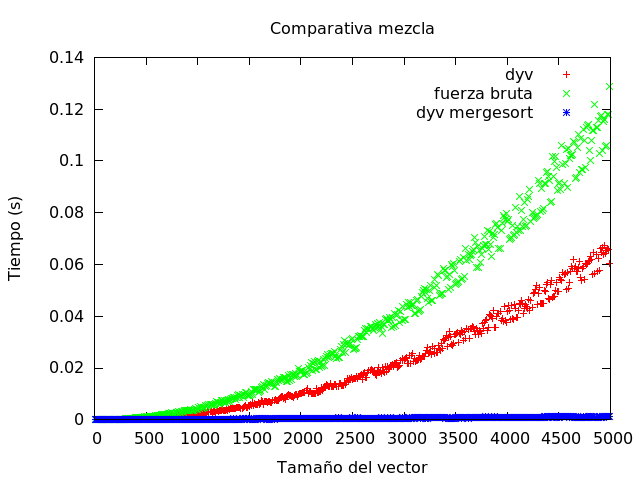
\includegraphics[width=0.6\textwidth]{../Opcional/Graficas/comparativa.png}
	\caption{Subproblemas} 
	\label{fig:perros} 
\end{figure}

